\documentclass[12pt,compress]{beamer}
\usepackage{ifthen}

\title{Status of \\ Track-based Muon Chamber Alignment}
\author{Jim Pivarski}
\institute{Texas A\&M University}
\date{14 November, 2006}

\setbeamertemplate{navigation symbols}{}
\setbeamertemplate{headline}{\includegraphics[height=1 cm]{../cmslogo} \hspace{0.1 cm} \includegraphics[height=1 cm]{../tamulogo} \hfill
\begin{minipage}{9 cm}
\vspace{-0.75 cm} \small
\begin{center}
\ifthenelse{\equal{\insertpagenumber}{1}}{}{\insertsection}
\end{center}
\end{minipage} \hfill
\begin{minipage}{1 cm}
\vspace{-0.75 cm} \small
\begin{center}
\ifthenelse{\equal{\insertpagenumber}{1}}{}{\insertpagenumber/\pageref{numpages}}
\end{center}
\end{minipage}}

\xdefinecolor{verylightgray}{rgb}{0.95,0.95,0.95}
\beamertemplateshadingbackground{verylightgray}{white}

\xdefinecolor{dkgreen}{rgb}{0.,0.5,0.}

\begin{document}
\frame{\titlepage}
\section*{Track-based Muon Alignment --- Jim Pivarski}

\begin{frame}
\frametitle{Overview}
\begin{itemize}\setlength{\itemsep}{0.25 cm}
\item I am extending CommonAlignmentProducer to
\begin{enumerate}[\alph{enumi}) ]
  \item move muon chambers
  \item calculate muon residuals
\end{enumerate}
such that existing algorithms apply to muons
\item Most of the infrastructure is already general
\begin{itemize}
\item muon and tracker inherit from the same classes
\item I change the input and the generic class is passed through the
  system
\end{itemize}
\item Progress has been smooth: partially updated local copy compiles
  and runs
\item I've tested each feature change, but not the whole system
\end{itemize}
\end{frame}

\begin{frame}
\frametitle{Details}
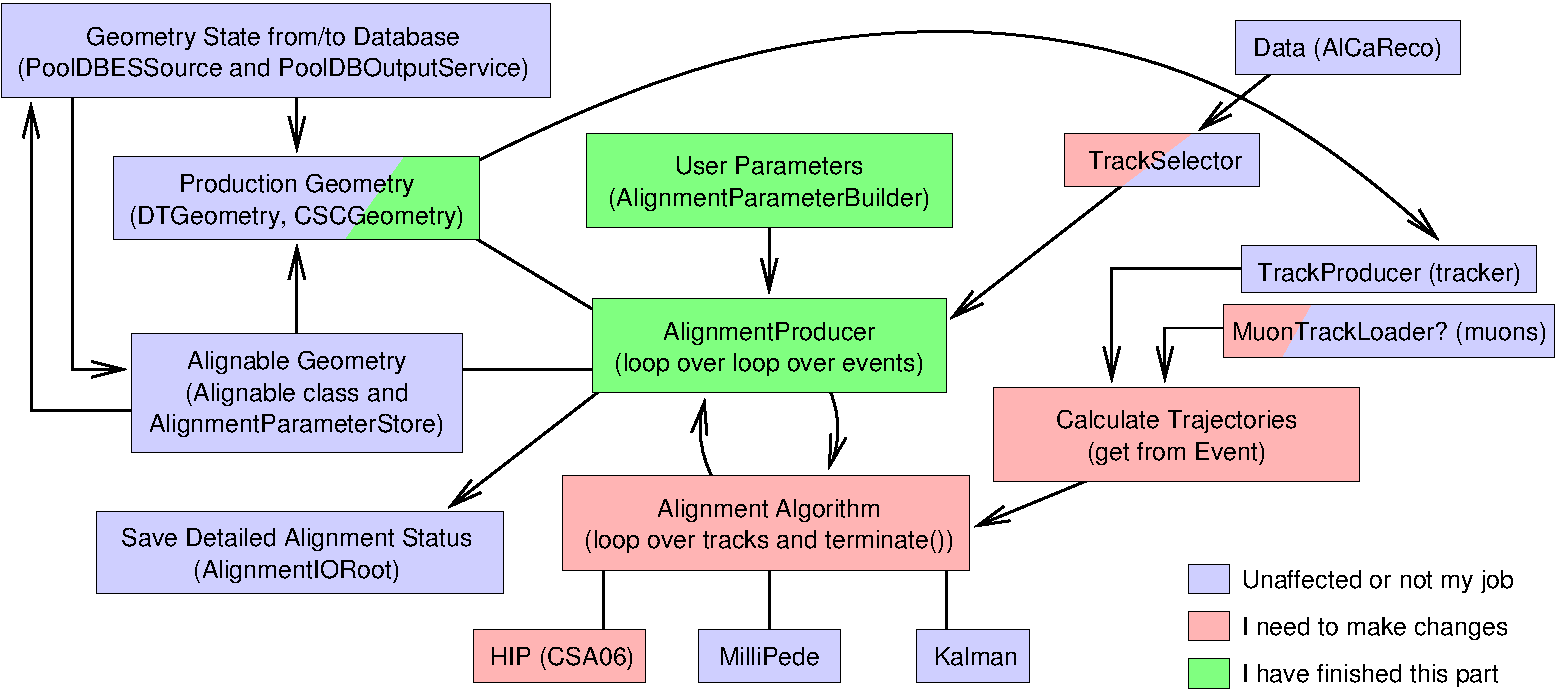
\includegraphics[width=\linewidth]{flow_chart}

\vfill
\only<2>{TrackSelector should require muon hits when doing muon alignment (easy)}
\only<3>{User Parameters: AlignmentParameterBuilder now selects muon
  Alignables, configurable with PSet \textcolor{dkgreen}{$\surd$}}
\only<4>{Production Geometry: DT(CSC)Geometry objects built by
  DT(CSC)GeometryBuilderFromDDD, not {\tt const} \textcolor{dkgreen}{$\surd$}}
\only<5>{Alignment corrections successfully applied from Alignable Geometry to
  Production Geometry \textcolor{dkgreen}{$\surd$}}
\only<6>{AlignmentProducer produces DT(CSC)Geometry (exports to Event) (still testing)}
\only<7>{All AlignmentAlgorithms need AlignableMuon* added to their
  initialize() argument lists (possibly other minor changes)}
\only<8>{Trajectories (for calculating residuals) may be loaded from
  Event, greatly simplifying existing code}
\end{frame}

\begin{frame}
\frametitle{Trajectories from Event}
\begin{itemize}\setlength{\itemsep}{0.75 cm}
\item Until recently, Trajectories could not be stored, so
  AlignmentAlgorithm recreated them with refitTracks()
\item Now they may be stored, we want to load with getByLabel()
\item MuonTrackLoader has PutTrajectoryIntoEvent parameter: perhaps
  this could be our refitter (e.g.\ for Kalman)?
\end{itemize}
\end{frame}

\begin{frame}
\frametitle{Updating All Three Algorithms}
\begin{itemize}\setlength{\itemsep}{0.5 cm}
\item I consider it my job to get CSA06AlignmentAlgorithm working for
  muons (testing and understanding the output)
\item MillePedeAlignmentAlgorithm loads Trajectories in the same way:
  update might be automatic (will be straightforward)
\item KalmanAlignmentAlgorithm refits Trajectories; may require
additional work or MuonTrackLoader
\end{itemize}

\vfill Updates to CSA06AlignmentAlgorithm provide a template for the
other two algorithms
\end{frame}

\begin{frame}
\frametitle{Plans}
\begin{enumerate}\setlength{\itemsep}{0.25 cm}
  \item Finish updating local copy of AlignmentProducer (1--2~weeks)
  \item Make sure CSA06AlignmentAlgorithm can do a muon chamber
  alignment (few weeks?)
  \item Carefully merge changes into CVS\ldots
\end{enumerate}

\vfill
\begin{enumerate}\setlength{\itemsep}{0.25 cm}\setcounter{enumi}{3}
  \item Expand monitoring of alignment procedure
  \item Branch off HIPAlignmentAlgorithm
\end{enumerate}
\label{numpages}
\end{frame}

\end{document}
